\chapter{\label{cha:qe_transquest}TransQuest: STS Architectures for QE}

\section{Introduction}
\cite{conneau-etal-2020-unsupervised} 

The main contributions of this chapter are as follows.
\begin{enumerate}
	\item We propose two architectures based on Transformers to perform sentence-level QE. These architectures are simpler than the predictor-estimator architecture which was the state-of-the-art in QE \cite{lee-2020-two, wang-etal-2018-alibaba}. 
	
	\item We evaluate them on both aspects of sentence-level QE on 15 language pairs and we show that the two architectures outperform the current state-of-the-art sentence-level QE frameworks like DeepQuest \cite{ive-etal-2018-deepquest} and OpenKiwi \cite{kepler-etal-2019-openkiwi}.
	
	\item We suggest further improvements to the models by data augmentation and ensemble learning.
	
	\item The findings of this chapter are published in \citet{ranasinghe-etal-2020-transquest}. 
	
	\item The two architectures introduced here was released as part of a QE framework; \textit{TransQuest}. TransQuest participated in WMT 2020 QE shared task 1\footnote{The shared task is available on \url{http://statmt.org/wmt21/quality-estimation-task.html}} \cite{specia-etal-2020-findings-wmt} and won it outperforming 50 teams around the globe \cite{ranasinghe-etal-2020-transquest-wmt2020}.
	
	\item The code and the pre-trained models of \textit{TransQuest} are publicly available to the community\footnote{The public GitHub repository is available on \url{https://github.com/tharindudr/TransQuest}. The pre-trained QE models for more than 15 language pairs are available on HuggingFace model repository on \url{https://huggingface.co/TransQuest}}. We have published \textit{TransQuest} as a python library\footnote{The developed python library is available on \url{https://pypi.org/project/transquest/}} and by the time of writing this chapter, it has more than 9,000 downloads from the community. 
	
\end{enumerate}

\section{Methodology}

As we mentioned before, we considered sentence-level QE as a crosslingual STS task. Therefore, we used the two best STS architectures we had in part I of the thesis. As we mentioned in Part I, these architectures were based on Transformers; the default sentence pair classification architecture in Transformers and the Siamese Transformer model described in \ref{cha:sts_transformers}. However, rather than using monolingual Transformers as in STS, we have to use crosslingual Transformers for the QE task, that can represent both languages in the same vector space.

Although there are several multilingual transformer models like multilingual BERT (mBERT) \cite{devlin-etal-2019-bert} and multilingual DistilBERT (mDistilBERT) \cite{Sanh2019DistilBERTAD}, researchers expressed some reservations about their ability to represent all the languages \cite{pires-etal-2019-multilingual}. In addition, although mBERT and mDistilBERT showed some crosslingual characteristics, they do not perform well on crosslingual benchmarks \cite{karthikeyan2020cross} as they have not being trained using crosslingual data. 

XLM-RoBERTa (XML-R) was released in November 2019 \cite{conneau-etal-2020-unsupervised} as an update to the XLM-100 model \cite{lample2019cross}. XLM-R takes a step back from XLM, eschewing XLM's Translation Language Modeling (TLM) objective since it requires a dataset of parallel sentences, which can be difficult to acquire. Instead, XLM-R trains RoBERTa\cite{liu2019roberta} on a huge, multilingual dataset at an enormous scale: unlabelled text in 104 languages, extracted from CommonCrawl datasets, totalling 2.5TB of text. It is trained using only RoBERTa's \cite{liu2019roberta} masked language modelling (MLM) objective. Surprisingly, this strategy provided better results in crosslingual tasks. XLM-R outperforms mBERT on a variety of crosslingual benchmarks such as crosslingual natural language inference and crosslingual question answering \cite{conneau-etal-2020-unsupervised}. This superior performance of XLM-R in crosslingual tasks motivated us to use XLM-R in QE. 

The \textit{TransQuest} framework that is used to implement the two architectures described here relies on the XLM-R transformer model \cite{conneau-etal-2020-unsupervised} to derive the representations of the input sentences. The XLM-R transformer model takes a sequence of no more than 512 tokens as input and outputs the representation of the sequence. The first token of the sequence is always \textsc{[CLS]}, which contains the special embedding to represent the whole sequence, followed by embeddings acquired for each word in the sequence. As shown below, our proposed neural network architectures can utilise both the embedding for the \textsc{[CLS]} token and the embeddings generated for each word. The output of the transformer (or transformers for \textit{SiameseTransQuest} described below), is fed into a simple output layer which is used to estimate the quality of a translation. We describe below the way the XLM-R transformer is used and the output layer, as they are different in the two instantiations of the framework. The fact that we do not rely on a complex output layer makes training our architectures much less computational intensive than state-of-the-art QE solutions like predictor-estimator \cite{lee-2020-two, wang-etal-2018-alibaba}.

There are two pre-trained XLM-R models released by HuggingFace's Transformers library \cite{wolf-etal-2020-transformers}; XLM-R-base and XLM-R-large. We used both of these architectures in our experiments\footnote{XLM-R-large is available on \url{https://huggingface.co/xlm-roberta-large} and XLM-R-base is available on \url{https://huggingface.co/xlm-roberta-base}}. Both of these pre-trained XLM-R models cover 104 languages \cite{conneau-etal-2020-unsupervised}, making it potentially very useful to estimate the translation quality for a large number of language pairs.

\begin{enumerate}
	\item \textbf{MonoTransQuest} (\textbf{MTransQuest}): 
	The first architecture proposed uses a single XLM-R transformer model and is shown in Figure \ref{fig:monotransquest}. This architecture produced the best results for monolingual STS tasks in Part I of the thesis. The input of this model is a concatenation of the original sentence and its translation, separated by the \textsc{[SEP]} token. We experimented with three pooling strategies for the output of the transformer model: using the output of the \textsc{[CLS]} token (\texttt{CLS}-strategy); computing the mean of all output vectors of the input words (\texttt{MEAN}-strategy); and computing a max-over-time of the output vectors of the input words (\texttt{MAX}-strategy). The output of the pooling strategy is used as the input of a softmax layer that predicts the quality score of the translation. We used mean-squared-error loss as the objective function. Early experiments we carried out demonstrated that the \texttt{CLS}-strategy leads to better results than the other two strategies for this architecture. Therefore,  we used the embedding of the \textsc{[CLS]} token as the input of a softmax layer.
	
	
	\item \textbf{SiameseTransQuest} (\textbf{STransQuest}): The second approach proposed in this paper relies on the Siamese architecture depicted in Figure \ref{fig:siamesetransquest} showed promising results in monolingual STS tasks \cite{reimers-gurevych-2019-sentence} in Part I of the thesis. In this case, we feed the original text and the translation into two separate XLM-R transformer models. Similar to the previous architecture we used the same three pooling strategies for the outputs of the transformer models. We then calculated the cosine similarity between the two outputs of the pooling strategy. We used mean-squared-error loss as the objective function. In initial experiments we carried out with this architecture, the \texttt{MEAN}-strategy showed better results than the other two strategies. For this reason, we used the \texttt{MEAN}-strategy for our experiments. Therefore, cosine similarity is calculated between the the mean of all output vectors of the input words produced by each transformer. 

	
\end{enumerate}


\begin{figure}[!ht]
	\centering
	\begin{subfigure}[b]{10cm}
		\centering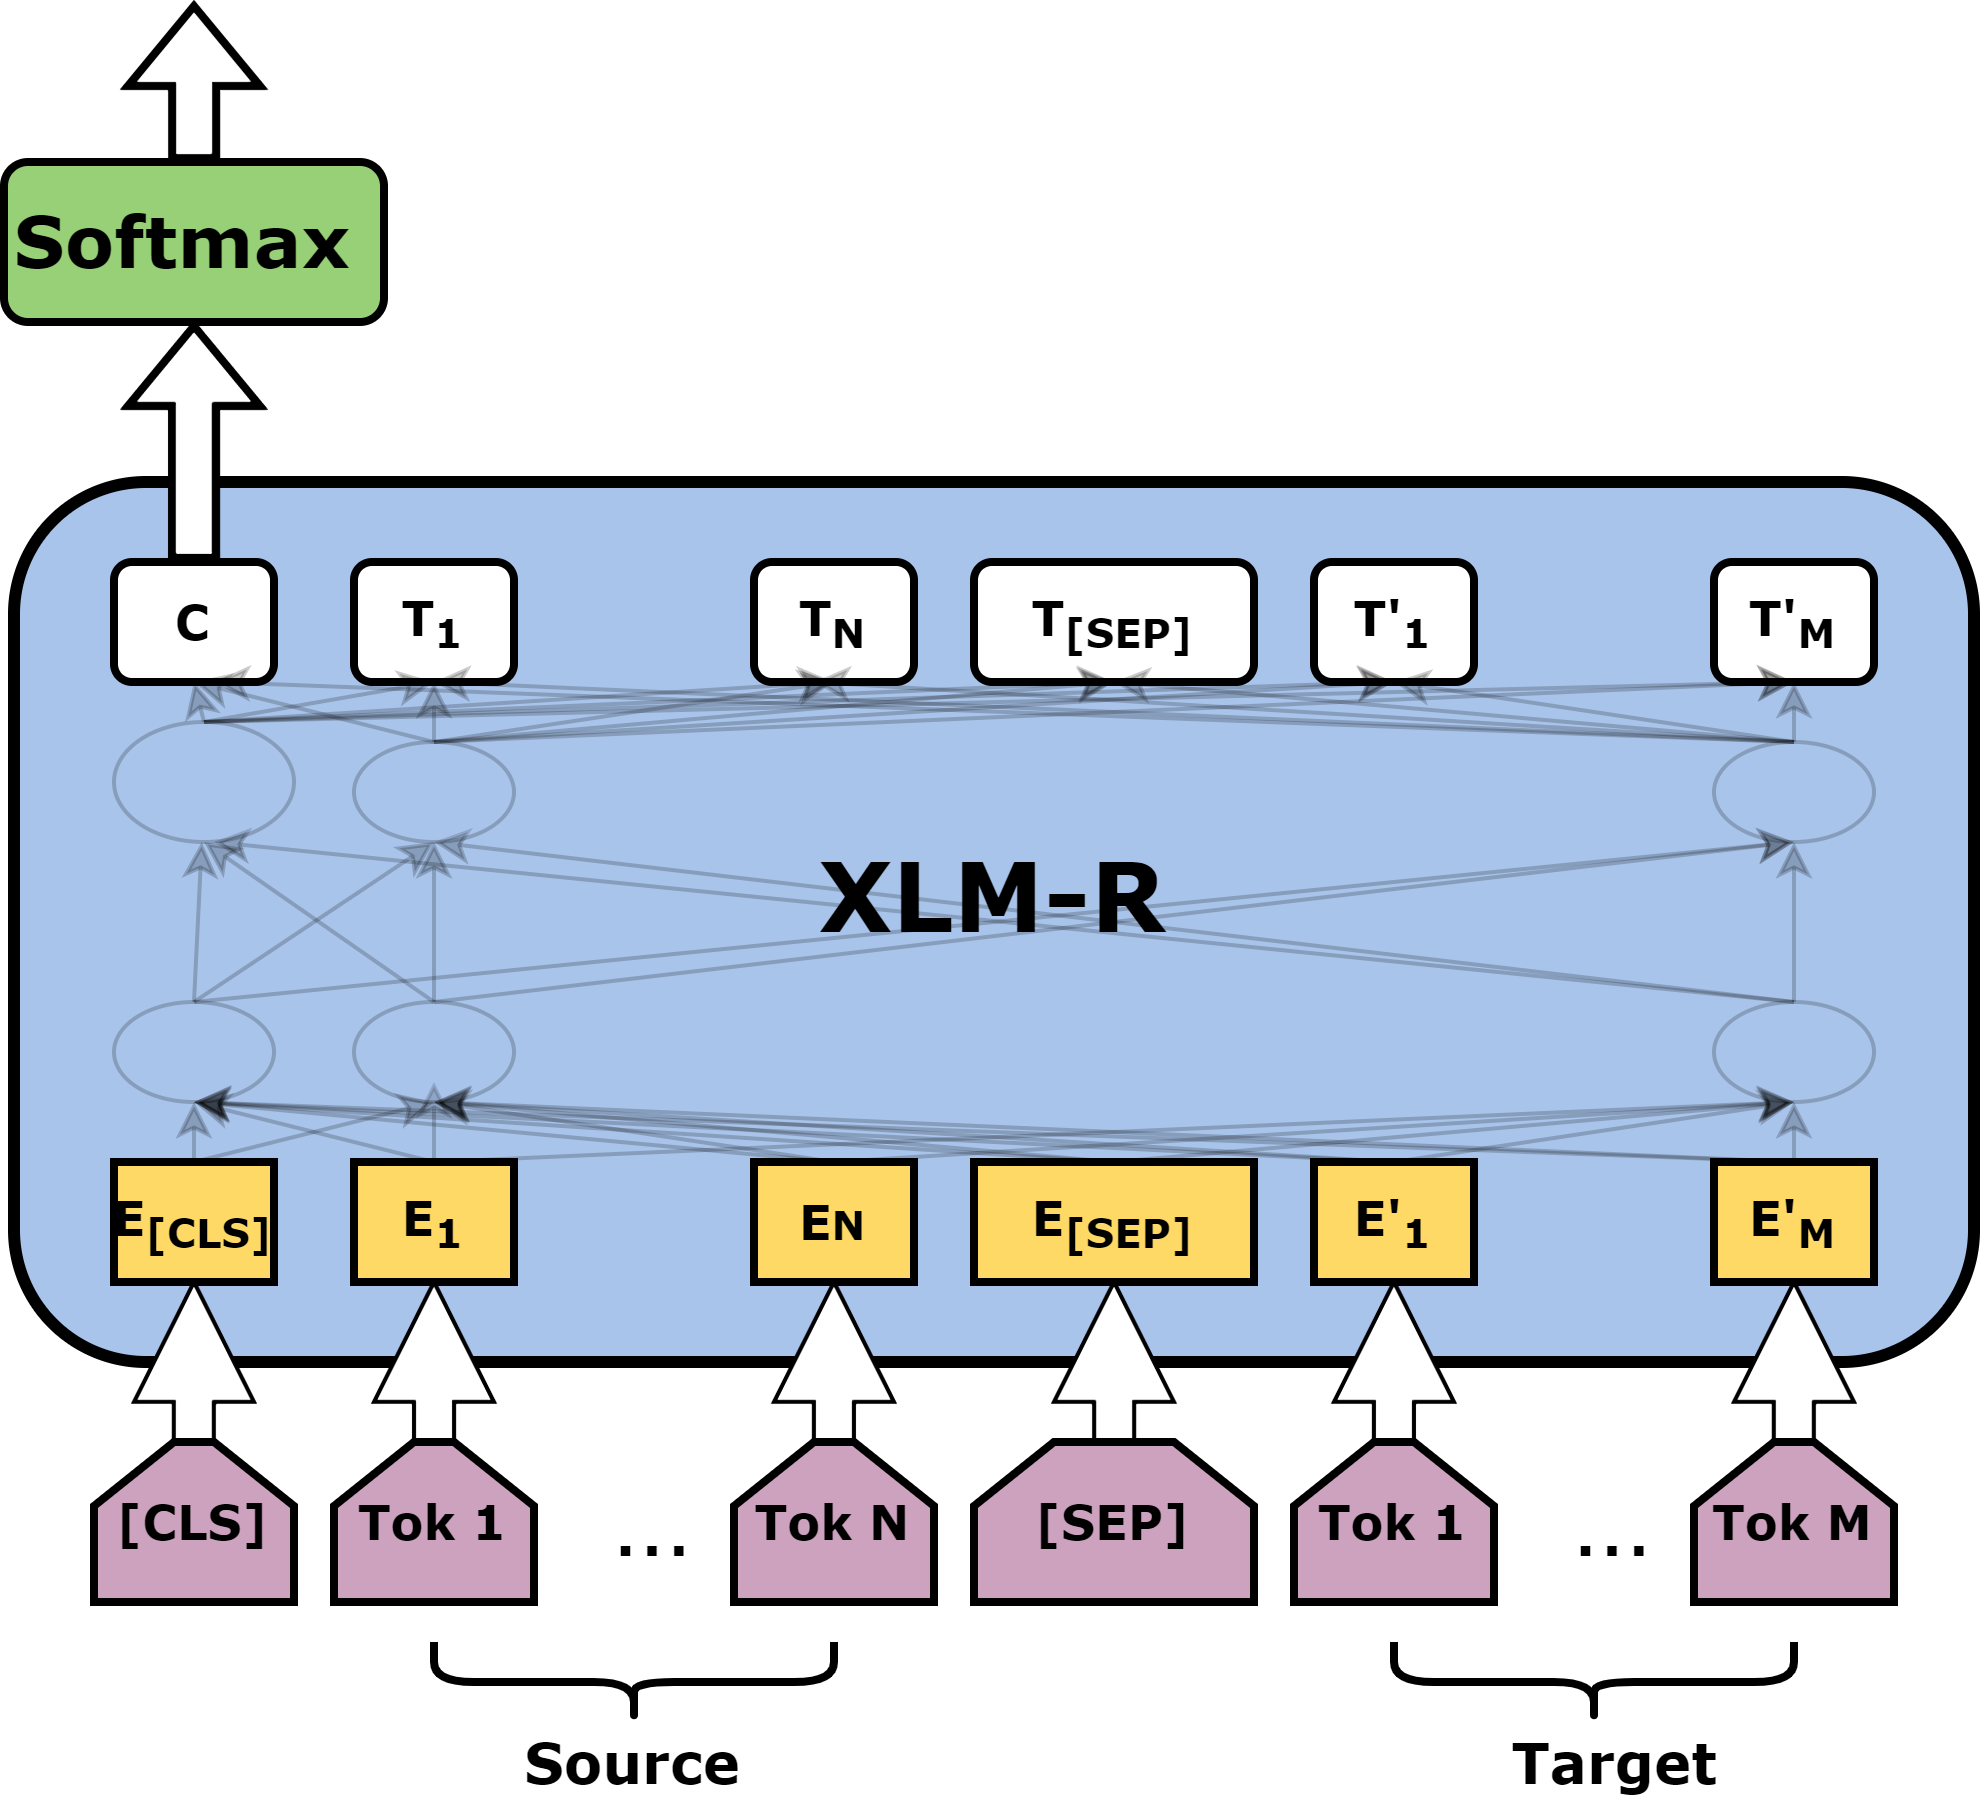
\includegraphics[width=8cm]{figures/translation_quality_estimation/TransQuest.png}
		\caption{\textit{MonoTransQuest} Architecture}
		\label{fig:monotransquest}
	\end{subfigure}
	\begin{subfigure}[b]{10cm}
		\centering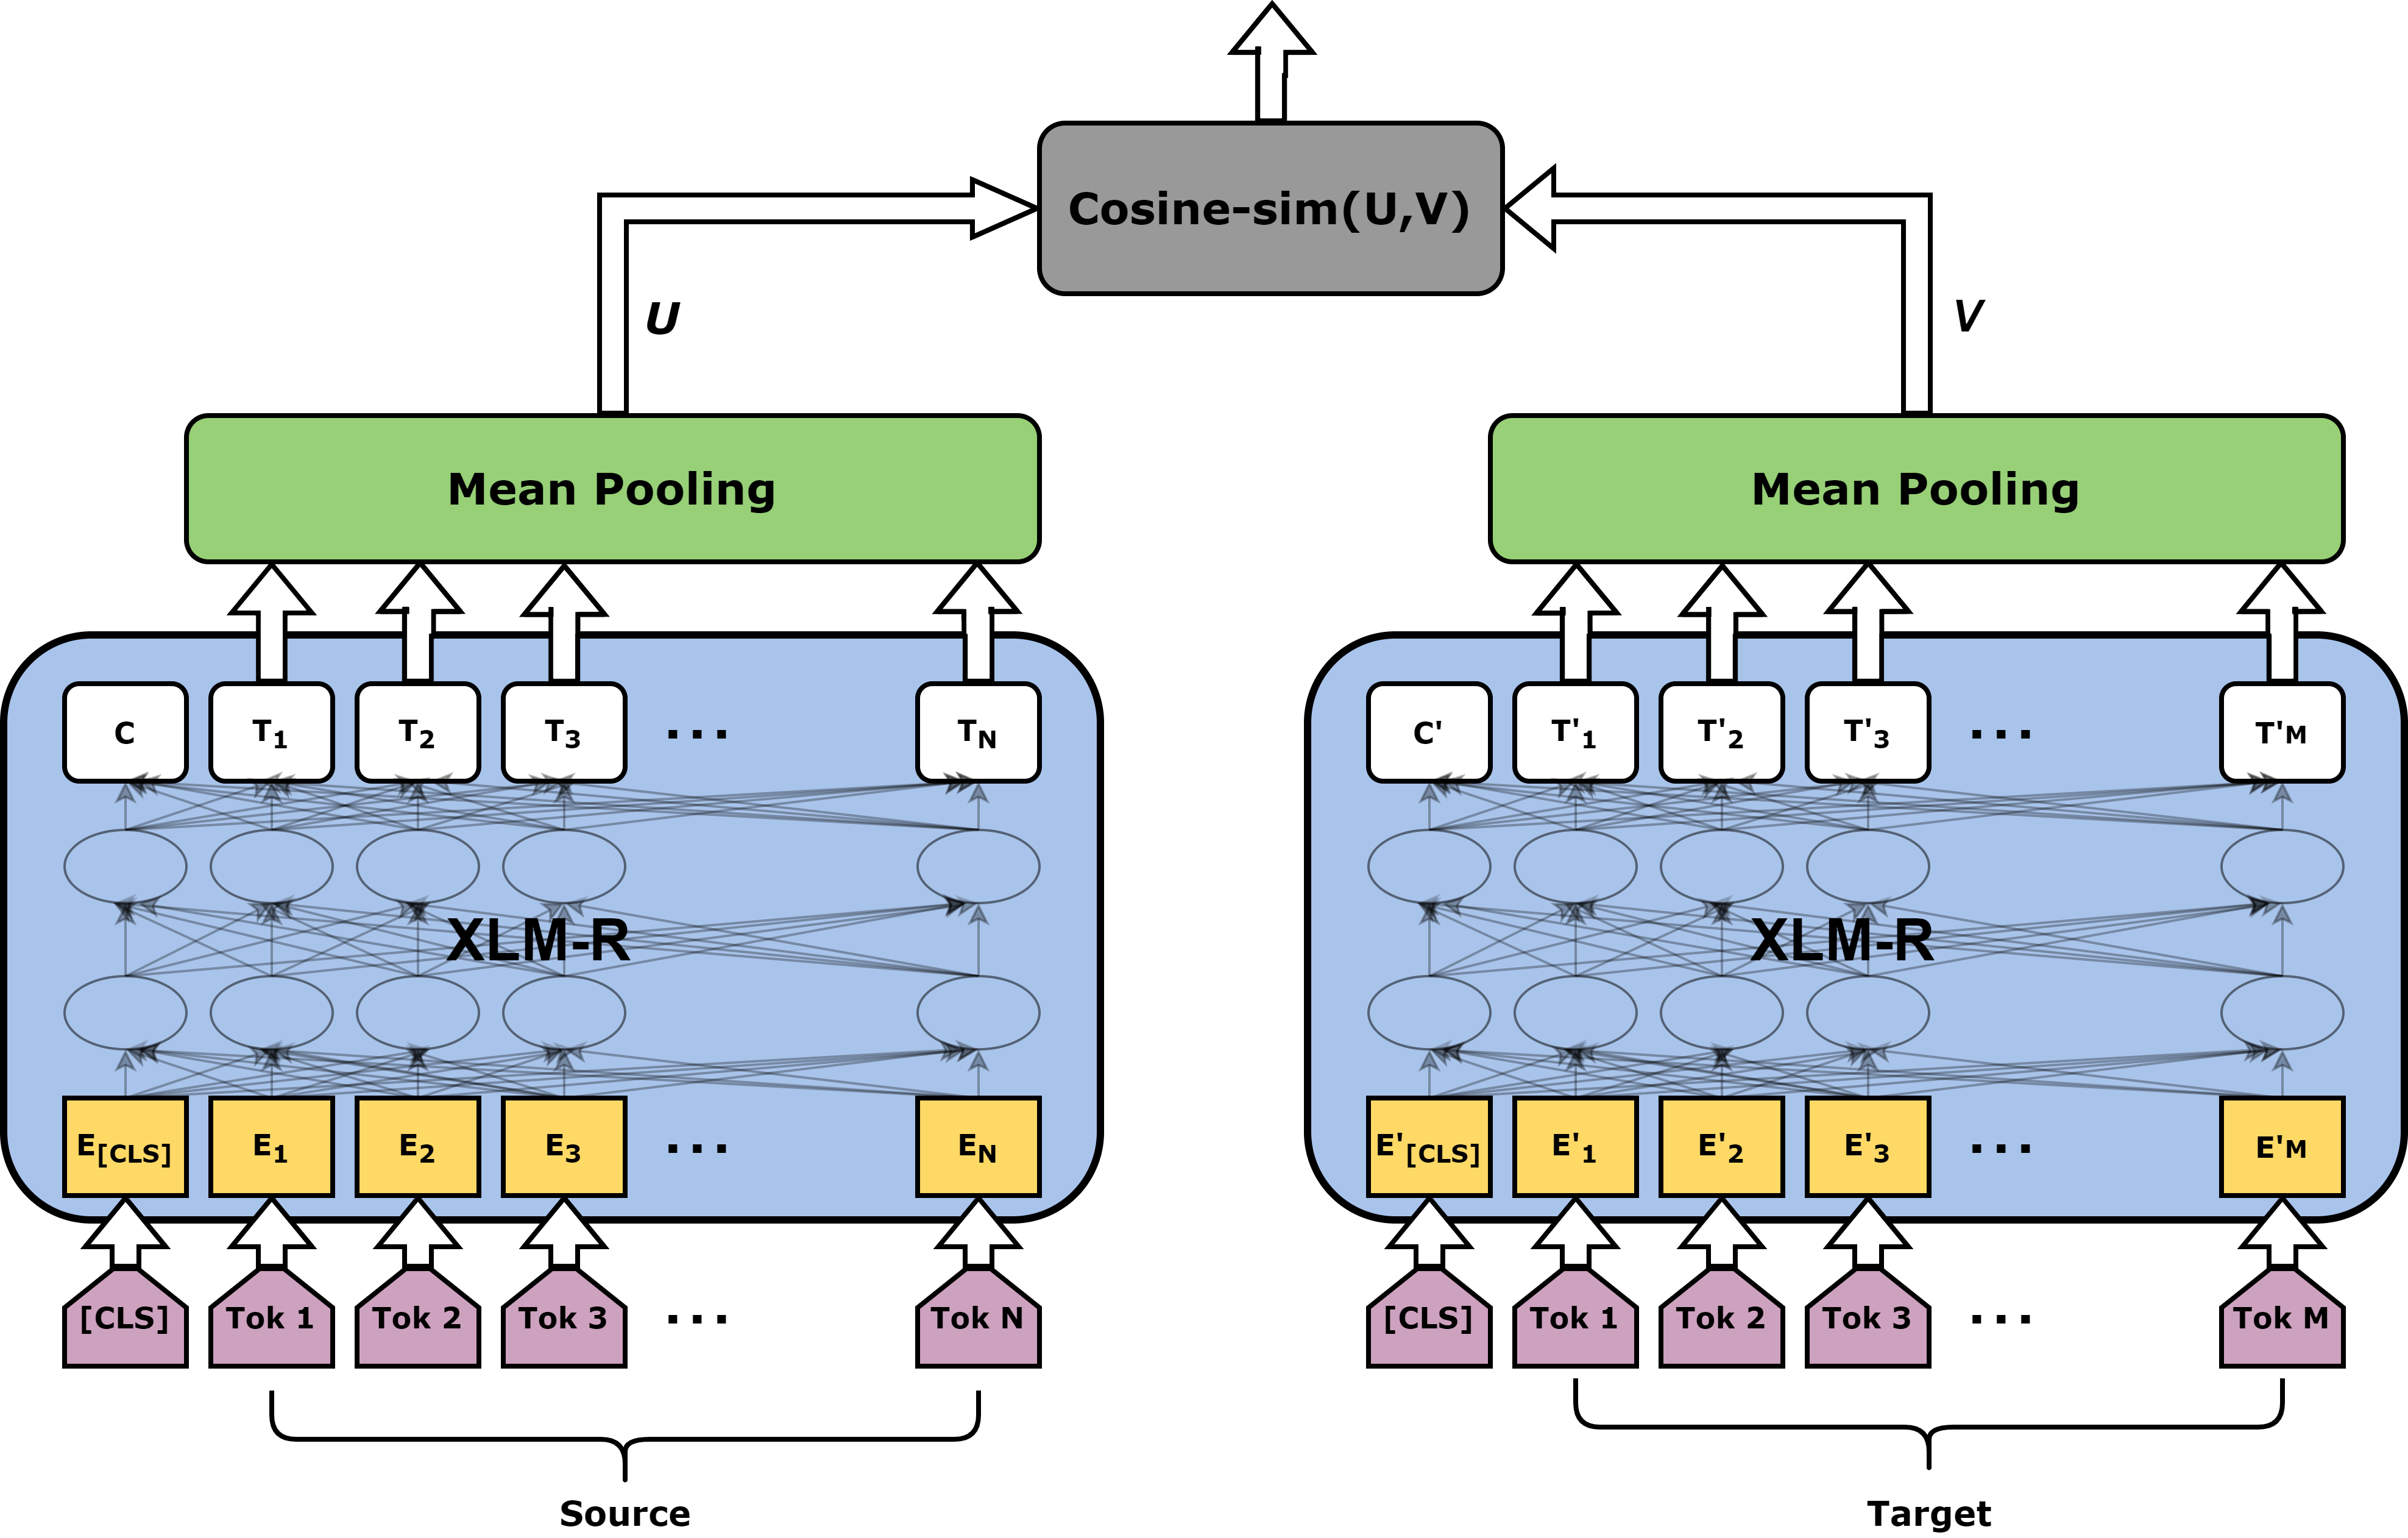
\includegraphics[width=12cm]{figures/translation_quality_estimation/SiameseTransQuest.png}
		\caption{\textit{SiameseTransQuest} Architecture}
		\label{fig:siamesetransquest}
	\end{subfigure}
	
	\caption[Architectures in TransQuest]{Two architectures employed in TransQuest.}
	\label{fig:transquest_architecture}
\end{figure}

\subsection{Experimental Setup}
We evaluated these two architectures in both aspects of sentence-level quality estimation using the data introduced in Chapter \ref{cha:qe_introduction}. We applied the same set of configurations for all the language pairs in order to ensure consistency between all the experiments. This also provides a good starting configuration for researchers who intend to use TransQuest on a new language pair. In both architectures we used a batch-size of eight, Adam optimiser with learning rate $2\mathrm{e}{-5}$, and a linear learning rate warm-up over 10\% of the training data. During the training process, the parameters of XLM-R model, as well as the parameters of the subsequent layers, were updated. The models were trained using only training data. Furthermore, they were evaluated while training once in every 300 training steps using an evaluation set that had one fifth of the rows in training data. We performed early stopping if the evaluation loss did not improve over ten evaluation steps. All the models were trained for three epochs.

\section{Results and Discussion}
The results for HTER and DA aspects are shown in Tables \ref{tab:hter_prediction} and \ref{tab:da_prediction}. We report the Pearson correlation ($\bm{\rho}$) between the predictions and the gold labels from the test set, which is the most commonly used evaluation metric in recent WMT quality estimation shared tasks \cite{specia-etal-2018-findings,fonseca-etal-2019-findings,specia-etal-2020-findings-wmt} as mentioned in Chapter \ref{cha:qe_introduction}. Since we use the same evaluation process, we could compare our results with the baselines and best systems of the respective shared task.

\renewcommand{\arraystretch}{1.2}
\begin{table}[t]
	\begin{center}
		\small
		% \footnotesize
		\scalebox{0.8}{
		\begin{tabular}{l l  c c c c c c c c} 
			%\hline
			\toprule
			& & \multicolumn{4}{c}{\bf Mid-resource} & \multicolumn{4}{c}{\bf High-resource}\\\cmidrule(r){3-6}\cmidrule(r){7-10}
			&{\bf Method} & \makecell{En-Cs \\ SMT} & \makecell{ En-Ru \\ NMT} & \makecell{En-Lv \\ SMT} & \makecell{En-Lv \\ NMT} & \makecell{De-En \\ SMT} & \makecell{En-Zh \\ NMT} & \makecell{En-De \\ SMT } & \makecell{En-De \\ NMT} \\
			\midrule
			\multirow{2}{*}{\bf I} & MTransQuest & 0.7207 & 0.7126 & 0.6592 & 0.7394 & 0.7939 & 0.6119 & 0.7137 & 0.5994\\
			& STransQuest & 0.6853 & 0.6723 & 0.6320 & 0.7183 & 0.7524 & 0.5821& 0.6992 & 0.5875 \\
			\midrule
			\multirow{2}{*}{\bf II} & MTransQuest-base & 0.7012 & 0.6982 & 0.6254 & 0.7110 & 0.7653 & 0.5873 & 0.6872 & 0.5762 \\
			& STransQuest-base & 0.6678 & 0.6542 & 0.6132 & 0.6892 & 0.7251 & 0.5551 & 0.6672 & 0.5532 \\
			\midrule
			\multirow{2}{*}{\bf III} & MTransQuest $\otimes$ & 0.7300 & 0.7226 & 0.6601 & 0.7402 & 0.8021 & 0.6289 & 0.7289 & 0.6091 \\
			& STransQuest $\otimes$ & 0.6901 & 0.6892 & 0.6451 & 0.7251 & 0.7649 & 0.5967& 0.7041 & 0.5991 \\
			\midrule
			\multirow{2}{*}{\bf IV} & MTransQuest $\otimes$ - Aug & \textbf{0.7399} & \textbf{0.7307} & \textbf{0.6792} & \textbf{0.7492} & \textbf{0.8109} & 0.6367 & \textbf{0.7398} & \textbf{0.6156}\\
			& STransQuest $\otimes$ - Aug & 0.7002 & 0.6901 & 0.6498 & 0.7301 & 0.7667 & 0.5991& 0.7134 & 0.6098 \\
			\midrule
			\multirow{3}{*}{\bf V} & Quest ++ & 0.3943 & 0.2601 & 0.3528 & 0.4435 & 0.3323 & NR & 0.3653 & NR \\
			& OpenKiwi & NR & 0.5923 & NR & NR & NR & 0.5058 & 0.7108 & 0.4001 \\
			& Best system & 0.6918 & 0.5923 & 0.6188 & 0.6819 & 0.7888 & \textbf{0.6641} & 0.7397 &  0.5718 \\
			\midrule
			\multirow{2}{*}{\bf VI} & MTransQuest-B & 0.6423 & 0.6354 & 0.5772 & 0.6531 & 0.7005 & 0.5483 & 0.6239 & 0.5002 \\
			& STransQuest-B & 0.5987 & 0.5872 & 0.5012 & 0.5901 & 0.6572 & 0.5098& 0.5762 & 0.4551 \\
			\bottomrule
			%\bottomrule
		\end{tabular}
	}
	\end{center}
	\caption[Pearson correlation between TransQuest algorithm predictions and human post-editing effort]{Pearson correlation ($\bm{\rho}$) between \textit{TransQuest} algorithm predictions and human post-editing effort. Best results for each language by any method are marked in bold. Row I shows the results for XLM-R-large model and Row II shows the results for XLM-R-base. Row III presents the results for further fine-tuning strategies explained in Section \ref{sec:transquest_finetune}. Row V shows the results of the baseline methods and the best system submitted for the language pair in that competition. \textbf{NR} implies that a particular result was \textit{not reported} by the organisers. Row VI presents the results of the multilingual BERT (mBERT) model in TransQuest Architectures.} 
	\label{tab:hter_prediction}
\end{table}



\renewcommand{\arraystretch}{1.2}
\begin{table*}[t]
	\begin{center}
		\small
		\scalebox{0.85}{
		\begin{tabular}{l l  c c c c c c c} 
			%\hline
			\toprule
			& & \multicolumn{2}{c}{\bf Low-resource} & \multicolumn{3}{c}{\bf Mid-resource} & \multicolumn{2}{c}{\bf High-resource}\\\cmidrule(r){3-4}\cmidrule(lr){5-7}\cmidrule(l){8-9}
			&{\bf Method} & Si-En & Ne-En & Et-En & Ro-En & Ru-En & En-De & En-Zh\\
			\midrule
			\multirow{2}{*}{\bf I} & MTransQuest & 0.6525 & 0.7914 & 0.7748 & 0.8982 & 0.7734 & 0.4669 & 0.4779 \\
			& STransQuest & 0.5957 & 0.7081 & 0.6804 & 0.8501 & 0.7126 & 0.3992 & 0.4067 \\
			\midrule
			\multirow{2}{*}{\bf II} & MTransQuest-base & 0.6412 & 0.7823 & 0.7651 & 0.8715 & 0.7593 & 0.4421 & 0.4593 \\
			& STransQuest-base & 0.5773 & 0.6853 & 0.6692 & 0.8321 & 0.6962 & 0.3832 & 0.3975 \\
			\midrule
			\multirow{2}{*}{\bf III} & MTransQuest $\otimes$ & 0.6661 & 0.8023 & 0.7876 & 0.8988 & 0.7854 & 0.4862 & 0.4853 \\
			& STransQuest $\otimes$ & 0.6001 & 0.7132 & 0.6901 & 0.8629 & 0.7248 & 0.4096 & 0.4159 \\
			\midrule
			\multirow{2}{*}{\bf IV} & MTransQuest $\otimes$ - Aug & \textbf{0.6849} & \textbf{0.8222} & \textbf{0.8240} & \textbf{0.9082} & \textbf{0.8082} & \textbf{0.5539} & \textbf{0.5373} \\
			& STransQuest $\otimes$ - Aug & 0.6241 & 0.7354 & 0.7239 & 0.8621 & 0.7458 & 0.4457 & 0.4658 \\
			\midrule
			\multirow{1}{*}{\bf V} & OpenKiwi & 0.3737 & 0.3860 & 0.4770 & 0.6845 & 0.5479 & 0.1455 & 0.1902 \\
			\midrule
			\multirow{2}{*}{\bf VI} & MTransQuest-B & NS & 0.6452 & 0.6231 & 0.8351 & 0.6661 & 0.3765 & 0.3982  \\
			& STransQuest-B & NS & 0.5368 & 0.5431 & 0.7652& 0.5541 & 0.3356 & 0.3462 \\
			\bottomrule
		\end{tabular}
	}
	\end{center}
	\caption[Pearson correlation ($\bm{\rho}$) between \textit{TransQuest} algorithm predictions and human DA judgments]{Pearson correlation ($\bm{\rho}$) between \textit{TransQuest} algorithm predictions and human DA judgments. Best results for each language (any method) are marked in bold. Row I shows the results for XLM-R-large model and Row II shows the results for XLM-R-base. Row III presents the results for further fine-tuning strategies explained in Section \ref{sec:transquest_finetune}. Row V shows the results of the baseline method; OpenKiwi. Row VI presents the results of the multilingual BERT (mBERT) model in TransQuest Architectures.} 
	\label{tab:da_prediction}
\end{table*}

In the HTER aspect of quality estimation, as shown in Table \ref{tab:hter_prediction}, \textit{MonoTransQuest} gains $\approx$ 0.1-0.2 Pearson correlation boost over OpenKiwi in most language pairs. In the language pairs where OpenKiwi results are not available \textit{MonoTransQuest} gains $\approx$ 0.3-0.4 Pearson correlation boost over QuEst++ in all language pairs for both NMT and SMT. Table \ref{tab:hter_prediction}  also gives the results of the best system submitted for a particular language pair. It is worth noting that the \textit{MonoTransQuest} results surpass the best system in all the language pairs with the exception of the En-De SMT and En-Zh NMT datasets. \textit{SiameseTransQuest} architecture too outperforms OpenKiwi and Quest++ in all the language pairs except En-De SMT. This shows that simple STS models with crosslingual embeddings outperforms the complex state-of-the-art QE models in HTER. 


As shown in Table \ref{tab:da_prediction}, in the DA aspect of quality estimation, \textit{MonoTransQuest}  gained $\approx$ 0.2-0.3 Pearson correlation boost over OpenKiwi in all the language pairs. Additionally, \textit{MonoTransQuest} achieves $\approx$ 0.4 Pearson correlation boost over OpenKiwi in the low-resource language pair Ne-En. \textit{SiameseTransQuest} too 

Additionally, row V in both Tables \ref{tab:hter_prediction} and \ref{tab:results:direct_assesement} shows the results of multilingual BERT (mBERT) in MonoTransQuest architecture. We used the same settings similar to XLM-R. The results show that XLM-R model outperforms the mBERT model in all the language pairs of both aspects in quality estimation and we can safely assume that the cross lingual nature of the XLM-R transformers had a clear impact to the results.

\subsection{Further Fine-tunning}
\label{sec:transquest_finetune}


\subsection{Error analysis}
\label{sebsec:error}

In an attempt to better understand the performance and limitations of \textit{TransQuest} we carried out an error analysis on the results obtained on Romanian - English and Sinhala - English. The choice of language pairs we analysed was determined by the availability of native speakers to perform this analysis. We focused on the cases where the difference between the predicted score and expected score was the greatest. This included both cases where the predicted score was underestimated and overestimated. 

Analysis of the results does not reveal very clear patterns. The largest number of errors seem to be caused by the presence of named entities in the source sentences. In some cases these entities are mishandled during the translation. The resulting sentences are usually syntactically correct, but semantically odd. Typical examples are \emph{RO: În urmă explorărilor Căpitanului James Cook, Australia și Noua Zeelandă au devenit ținte ale colonialismului britanic. (As a result of Captain James Cook's explorations, Australia and New Zealand have  become the targets of British colonialism.)} - \emph{EN: Captain James Cook, Australia and New Zealand have finally become the targets of British colonialism.} (expected: -1.2360, predicted: 0.2560) and \emph{RO: O altă problemă importantă cu care trupele Antantei au fost obligate să se confrunte a fost malaria. (Another important problem that the Triple Entente troops had to face was malaria.)} - EN: \emph{Another important problem that Antarctic troops had to face was malaria.} (expected: 0.2813, predicted: -0.9050). 
In the opinion of the authors of this paper, it is debatable whether the expected scores for these two pairs should be so different. Both of them have obvious problems and cannot be clearly understood without reading the source. For this reason, we would expect that both of them have low scores. Instances like this also occur in the training data. As a result of this, it may be that \textit{TransQuest} learns contradictory information, which in turn leads to errors at the testing stage.

A large number of problems are caused by incomplete source sentences or input sentences with noise. For example the pair \emph{RO: thumbright250pxDrapelul cu fâșiile în poziție verticală (The flag with strips in upright position)} -  \emph{EN: ghtghtness 250pxDrapel with strips in upright position} has an expected score of 0.0595, but our method predicts -0.9786. Given that only \emph{ghtghtness 250pxDrapel} is wrong in the translation, the predicted score is far too low. In an attempt to see how much this noise influences the result, we run the system with the pair \emph{RO: Drapelul cu fâșiile în poziție verticală} -  \emph{EN: Drapel with strips in upright position}. The prediction is 0.42132, which is more in line with our expectations given that one of the words is not translated. 

Similar to Ro-En, in Si-En the majority of problems seem to be caused by the presence of named entities in the source sentences. For an example in the English translation: \emph{But the disguised Shiv will help them securely establish the statue.
} (expected: 1.3618, predicted: -0.008), the correct English translation would be \emph{But the disguised Shividru will help them securely establish the statue.}. Only the named entity \emph{Shividru} is translated incorrectly, therefore the annotators have annotated the translation with a high quality. However TransQuest fails to identify that. Similar scenarios can be found in English translations \emph{Kamala Devi Chattopadhyay spoke at this meeting, Dr. Ann.} (expected:1.3177, predicted:-0.2999) and \emph{The Warrior Falls are stone's, halting, heraldry and stonework rather than cottages. The cathedral manor is navigable places} (expected:0.1677, predicted:-0.7587). It is clear that the presence of the named entities seem to confuse the algorithm we used, hence it needs to handle named entities in a proper way.




\section{Conclusion}